% vim: set foldmethod=marker foldlevel=0:

\documentclass[a4paper]{article}
\usepackage[UKenglish]{babel}

% NOTE: hyperref has to come before preamble
\usepackage{hyperref}

\usepackage{preamble}

\usepackage{graphicx}
\graphicspath{ {./imgs/} }

\fancyhead[L]{MA144 Assignment 1}
\title{MA144 Methods of Mathematical Modelling 2, Assignment 1}
\colorlet{questionbodycolor}{green!50}

\begin{document}

\maketitle

\setlength{\parindent}{0em}
\setlength{\parskip}{1em}

% {{{ Q1
\question{1}

\begin{questionbody}
Consider the polar curve with equation $r = f(\theta)$, where $\theta \in [a, b]$ and $f$ is some function of $\theta$.
\end{questionbody}

\subsection{~} % 1.a

\begin{questionbody}
Using the arc-length formula for parametric curves (in the lecture notes), show that the arc length of the polar curve is given by the integral \[
\intlim a b {\sqrt{\l( \dd f \theta \r)^2 + f^2}} \theta .
\]
\end{questionbody}

The polar curve with equation $r = f(\theta)$ can be parametrised as $\ul r (\theta) = (f(\theta) \cos \theta, f(\theta) \sin \theta)$. Then $$\dd{\ul r}\theta = \l(\dd f\theta (\theta) \cos \theta - f(\theta) \sin \theta, \dd f\theta (\theta) \sin \theta + f(\theta) \cos \theta\r)$$
Therefore \begin{align*}
\| \ul r\,'(\theta) \| &= \sqrt{\l( f'(\theta) \cos \theta - f(\theta) \sin \theta \r)^2 + \l( f'(\theta) \sin \theta + f(\theta) \cos \theta \r)^2}\\[1ex]
&= \sqrt{f'(\theta)^2 \cos^2 \theta - 2 f(\theta) f'(\theta) \cos\theta \sin\theta + f(\theta)^2 \sin^2 \theta}\\[1ex]
&\phantom{=} \overline{+ f'(\theta)^2 \sin^2 + 2 f(\theta) f'(\theta) \cos\theta \sin\theta + f(\theta)^2 \cos^2 \theta}\\[1ex]
&= \sqrt{f'(\theta)^2 (\cos^2 \theta + \sin^2 \theta) + f(\theta)^2 (\cos^2 \theta + \sin^2 \theta)}\\[1ex]
&= \sqrt{f'(\theta)^2 + f(\theta)^2}\\[1ex]
&= \sqrt{\l(\dd f\theta\r)^2 + f^2}\\[1ex]
\end{align*}

Therefore the arc length of the curve is $$s = \intlim ab {\sqrt{\l(\dd f\theta\r)^2 + f^2}}\theta$$ as required.

\subsection{~} % 1.b

\begin{questionbody}
Sketch the closed curve with polar equation $r = 1 + \cos \theta$. Find its arc length.
\end{questionbody}

\begin{figure}[h]
	\centering
	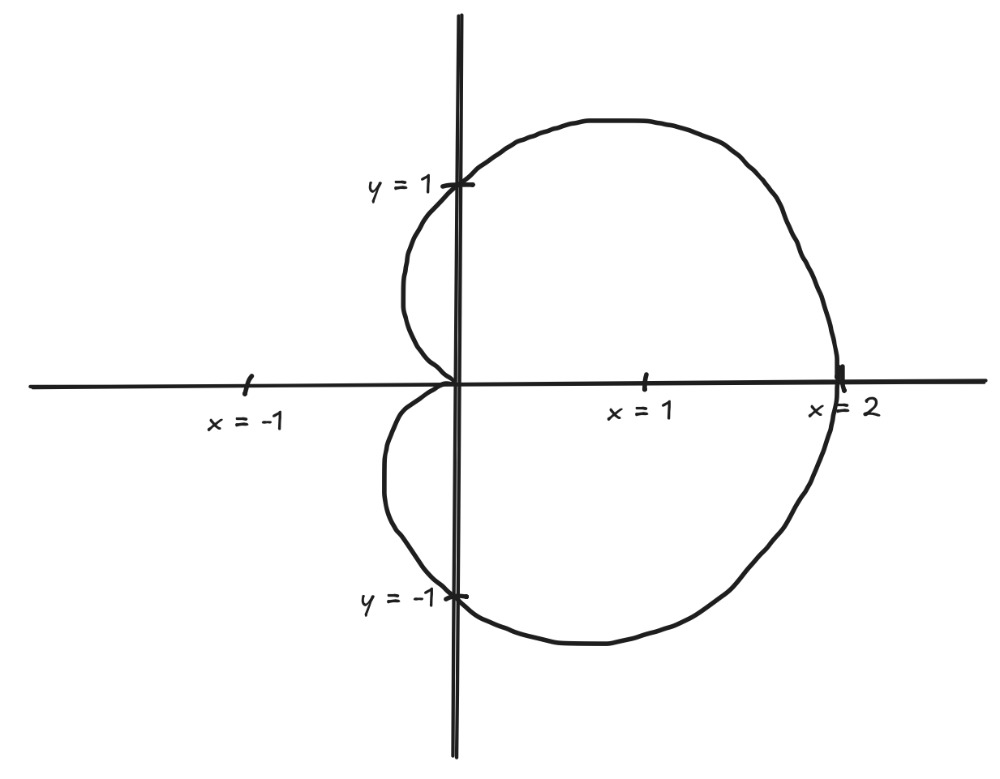
\includegraphics[scale=0.3]{Q1b}
	\caption{A sketch of $r = 1 + \cos\theta$}
\end{figure}

$\ds\dd r\theta = -\sin\theta$ so the arc length is \begin{align*}
s &= \intlim 0{2\pi} {\sqrt{\sin^2 \theta + (1 + \cos\theta)^2}} \theta\\[1ex]
&= \intlim 0{2\pi} {\sqrt{\sin^2 \theta + 1 + 2\cos\theta + \cos^2 \theta}} \theta\\[1ex]
&= \intlim 0{2\pi} {\sqrt{2 + 2\cos\theta}} \theta
\end{align*}
% TODO: Do this integral by hand
I don't know how to do this integral but apparently it's $4\pi$.

\newpage
\subsection{~} % 1.c

\begin{questionbody}
Consider the curve with polar equation $r = 1 + \cos k \theta$, where $\theta \in \R$. Give a value of the constant $k$ such that the curve is not simple. Justify your answer.
\end{questionbody}

% TODO: Justify this
The curve given by $r = 1 + \cos k\theta$ is non-simple (self-intersecting) whenever $k$ is not an integer.
% }}}

% {{{ Q2
\newquestion{2}

\begin{questionbody}
Consider the curve $\cal C$ with equation \[
\quad 4y^2 - 9x^2 = 1, \quad y > 0
\]
\end{questionbody}

\subsection{~} % 2.a

\begin{questionbody}
Parametrise the curve in terms of hyperbolic functions of $t$. Is this a regular parametrisation of the curve?
\end{questionbody}

Since $\cosh^2 t - \sinh^2 t = 1$, we can let $y = \f12 \cosh t$ and $x = \f13 \sinh t$. Then we'll have the equation of $\cal C$. Therefore we can parametrise $\cal C$ as $\ul r(t) = \l( \f13 \sinh t, \f12 \cosh t \r)$.

Since $\f12 \cosh t > 0$ for all $t \in (-\infty, \infty)$, the requirement of $y>0$ is satisfied by $t \in (-\infty, \infty)$, so that's the range of this parametrisation.

\subsection{~} % 2.b

\begin{questionbody}
Sketch the curve described by your parametrisation (include an arrow to indicate its orientation). Give the equations of any asymptotes.
\end{questionbody}

\begin{figure}[h]
	\centering
	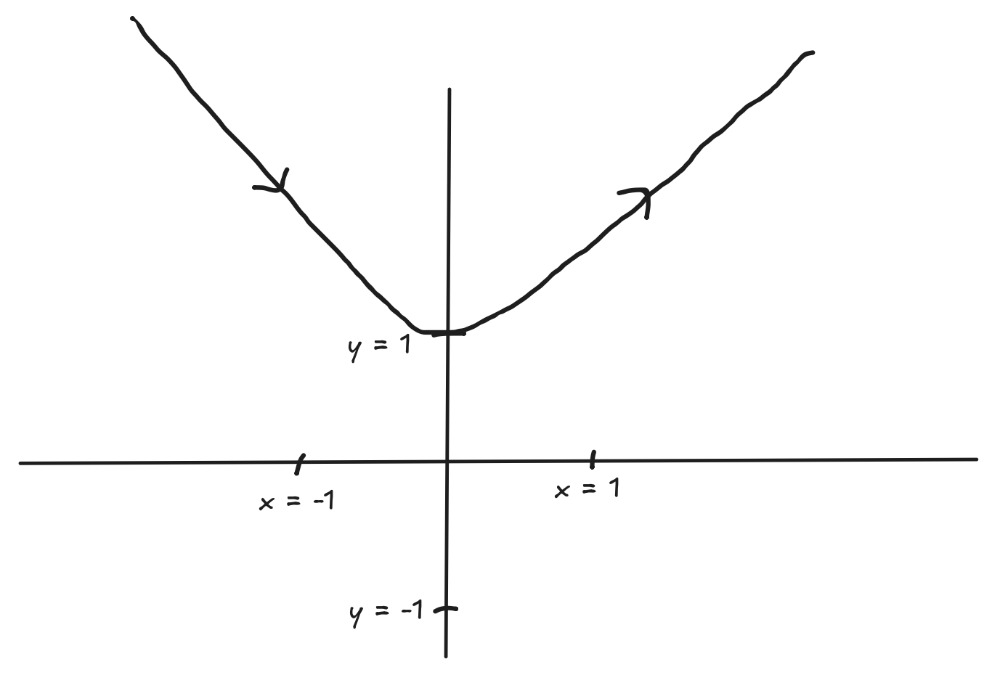
\includegraphics[scale=0.3]{Q2b}
	\caption{A sketch of $\ul r(t) = \l( \f13 \sinh t, \f12 \cosh t \r)$}
\end{figure}

There is a turning point at $\l(0, \f12\r)$ and asymptotes are $y = \f32 x$ and $y = -\f32 x$.

\newpage
\subsection{~} % 2.c

\begin{questionbody}
Write down a parametrisation of the curve using parameter $u$ such that $0 < u < 1$.
\end{questionbody}

To reparametrise with $u$ such that the bounds on the parametrisation are $u \in (0, 1)$, we want to adjust $t$ in the old parametrisation. We want $u = \f12$ when $t = 0$, $u \to 1$ as $t \to \infty$, and $u \to 0$ as $t \to \infty$. We want an increasing, sigmoid-shaped curve with horizontal asymptotes at $y=0$ and $y=1$. $\tanh$ almost fits this shape, but needs minor adjustments.

Let $u = \df{1 + \tanh t}2$. Then $u = \f12$ when $t = 0$, $u \to 1$ as $t \to \infty$, and $u \to 0$ as $t \to \infty$, as required. We rearrange to get $t = \artanh(2u - 1)$ and plug this into the old parametrisation.

Therefore $\cal C$ can also be parametrised as $$\l( \f13 \sinh\l(\artanh(2u - 1)\r), \f12 \cosh\l(\artanh(2u - 1)\r) \r) \quad u \in (0, 1)$$

We can also remove the hyperbolic functions and write it as $$\l( \f{2u-1}{6\sqrt{u - u^2}}, \f1{4\sqrt{u - u^2}} \r) \quad u \in (0, 1)$$
% }}}

% {{{ Q3
\newquestion{3}

\begin{questionbody}
A circle radius $r < 1$ is rolling on the inside of a circle radius 1, centred at the origin $O$. The centre $C$ of the smaller circle is initially at $(1 - r, 0)$. Let $\theta$ be the angle subtended by the line $OC$ measured with respect to the positive $x$ axis. The point $P$, initially at $(1, 0)$, traces out a curve as the smaller circle rolls inside the unit circle.

The curve traced out by $P$ has the parametric equations: \begin{align*}
x(\theta) &= (1 - r) \cos \theta + r \cos \l( \f{1-r}r \theta \r) , \\
y(\theta) &= (1 - r) \sin \theta - r \cos \l( \f{1-r}r \theta \r) .
\end{align*}
\end{questionbody}

\subsection{~} % 3.a

\begin{questionbody}
Use Python to plot the curves corresponding to $r = \f12, \f14, \f23$, and $\f1{\sqrt2}$, where $\theta \in [0, 10\pi]$. Plot them in 4 separate figures.
\end{questionbody}

\begin{figure}[hbtp]
	\centering
	\begin{tabular}{cc}
		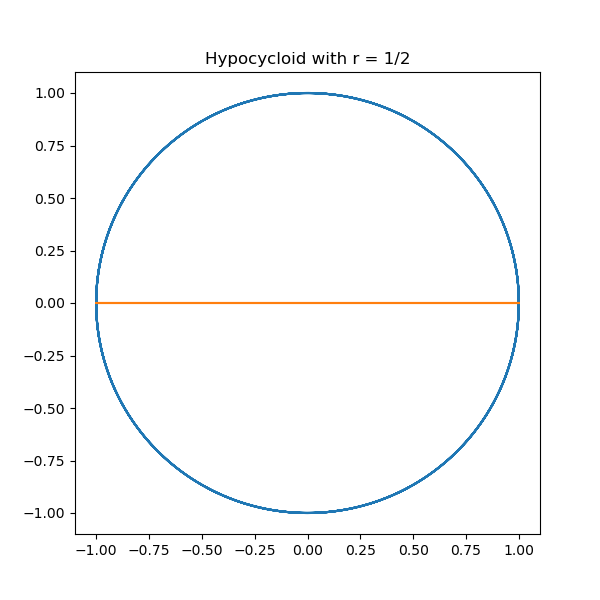
\includegraphics[scale=0.4]{Q3a-1} & 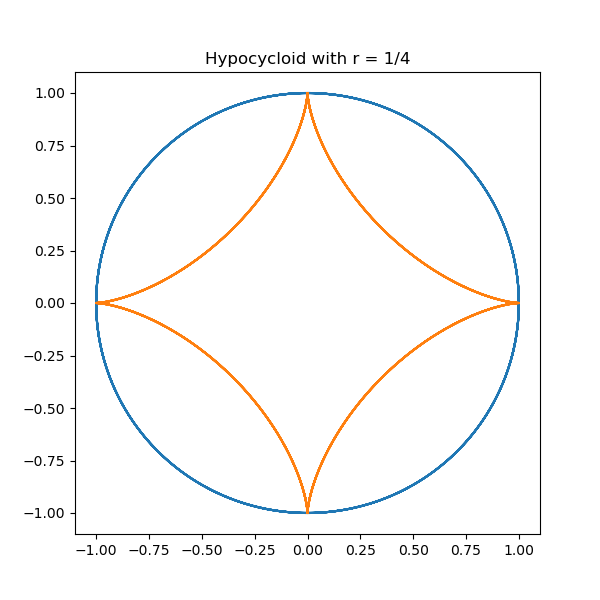
\includegraphics[scale=0.4]{Q3a-2}\\
		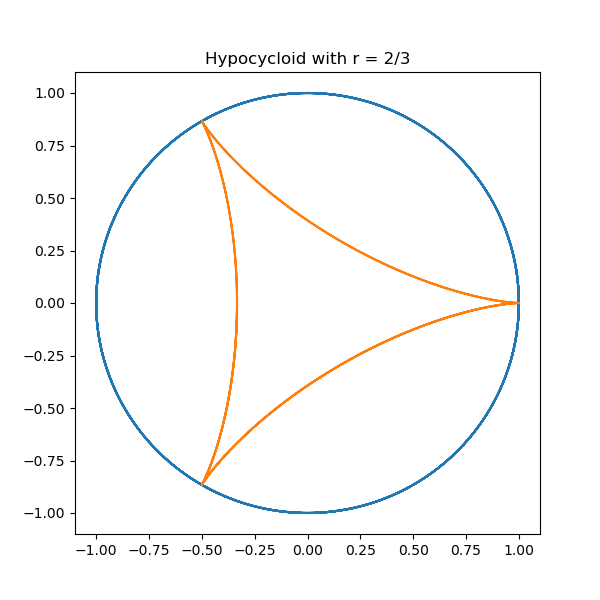
\includegraphics[scale=0.4]{Q3a-3} & 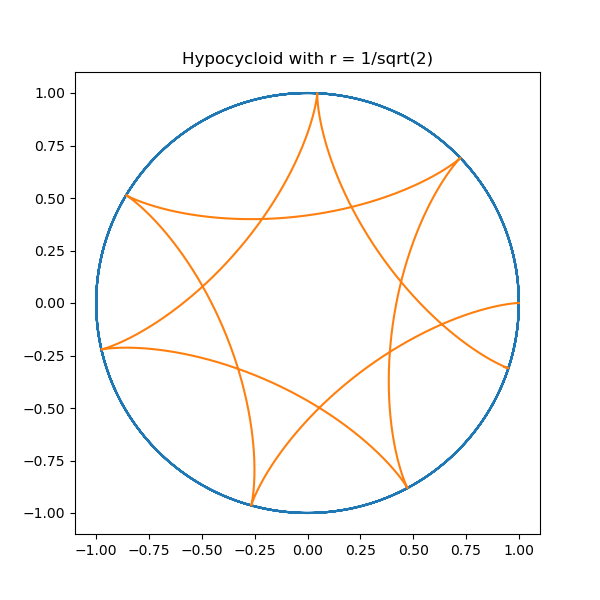
\includegraphics[scale=0.4]{Q3a-4}
	\end{tabular}
	\caption{Plots of hypocycloids for various values of $r$}
	\label{fig:hypocycloid-plots}
\end{figure}

\begin{figure}[hbtp]
	\centering
	\inputminted{python}{./code/generate_plots.py}
	\caption{The code used to generate the plots in Figure~\ref{fig:hypocycloid-plots}. The code can also be found \href{https://github.com/DoctorDalek1963/uni/blob/fe244f6880c7df0d801d426ca7ef9149b585ec2f/first-year/MA144-Methods-of-Mathematical-Modelling-2/Ass 1/code/generate_plots.py}{on GitHub}}
\end{figure}

\subsection{~} % 3.b

\begin{questionbody}
Make one conjecture on the appearance of the curve for an arbitrary $r \in \R$.
\end{questionbody}

I conjecture that for any $r \in \R$, the curve will be closed if and only if $r \in \Q$.
% }}}

\end{document}
